%
%  Chapter:  2 - Nuclear Models for High Spin Phenomena
%  Modified: 2/16/2015
%  Author:   James Till Matta
%
%%%%%%%%%%%%%%%%%%%%%%%%%%%%%%%%%%%%%%%%%%%%%%%%%%%%%%%%%%

\chapter{NUCLEAR MODELS FOR HIGH SPIN PHENOMENA}
\label{chp:models}

\section{Introduction}
\label{sec:models-into}
The atomic nucleus, discovered in $1911$ by Ernest Rutherford \cite{rutherfordNuclearModel}, is a tiny point of matter at the heart of an atom. This point of matter, is approximately $1-10fm$ across, contains more than $99.94\%$ of an atom's mass, and is composed of protons and neutrons. Since its discovery the nucleus has been studied and characterized using ever more sophisticated models.

Despite the sophistication of modern nuclear models, the task of nuclear modeling started from humble beginnings. Seeking to explain and predict nuclear properties several basic facts were gleaned from the observations at hand in that time. The strength and short range nature of the nuclear force is among the first and most important of these properties. The nuclear force had to be very strong indeed to overcome the coulomb repulsion of the protons in the nucleus, but its range had to be not much further than the radius of the nucleus due to its lack of impact on atomic phenomena. The nuclear forces range can be constrained yet further to nearest neighbors when one considers the saturation of the nuclear density (seen in Figure \ref{fig:chp2-density}) and binding energy per nucleon (seen in Figure \ref{fig:chp2-bpa}).

\begin{figure}
\label{fig:chp2-density}
\centerline{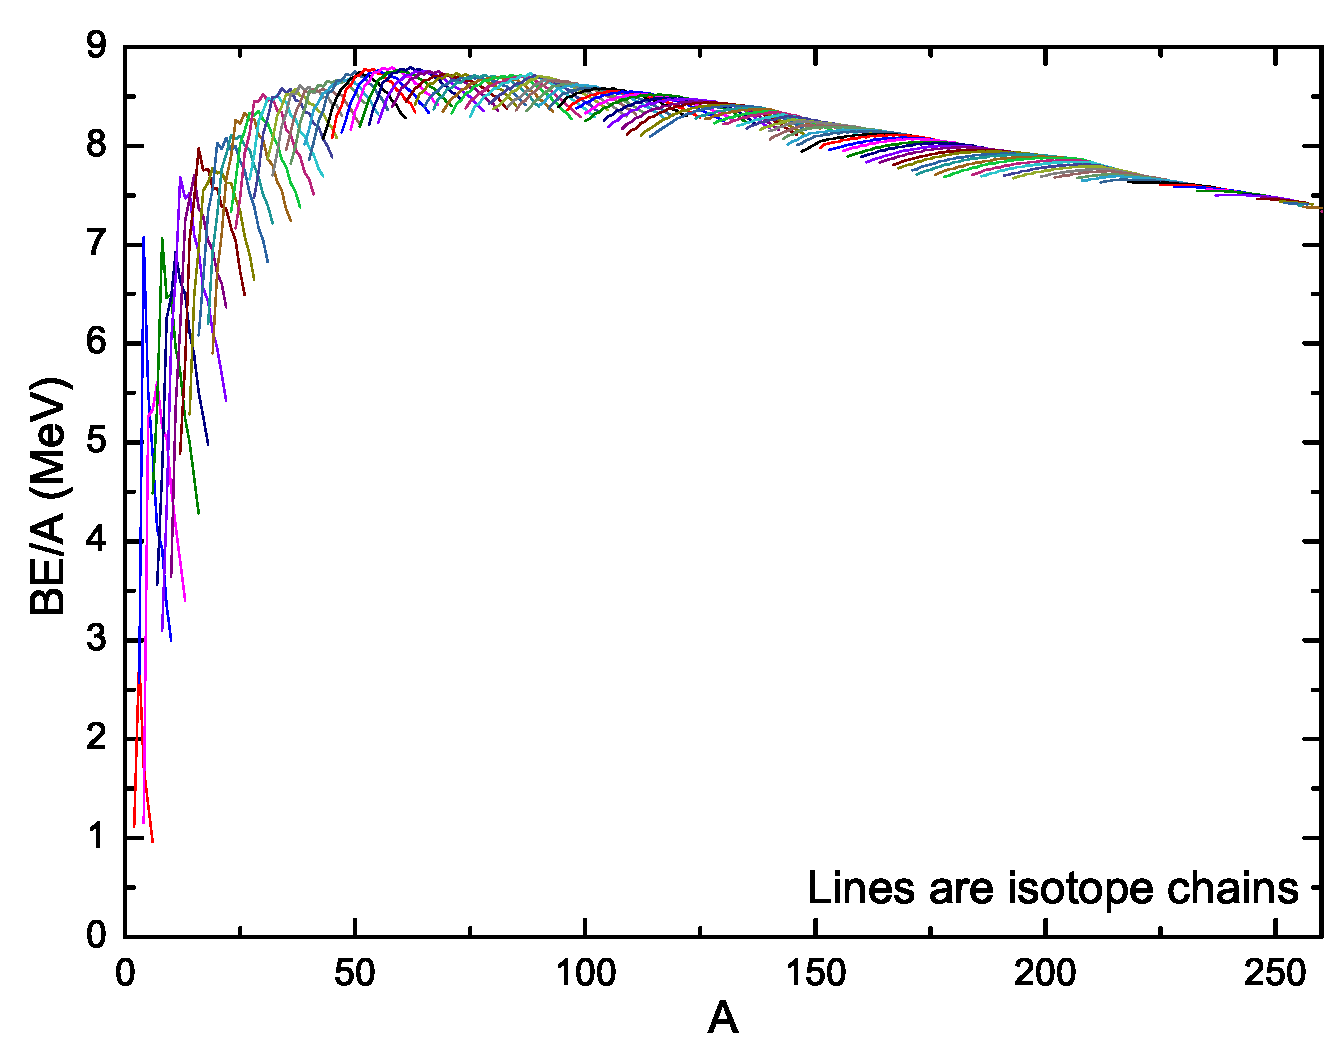
\includegraphics[width=\textwidth]{./img/c2/binding_plot.eps}}
	\caption{Binding energy per nucleon for every known isotope chain. Note the saturation starts in the $A\sim15-30$ region. Values calculated from: Ref. \cite{AME20031,AME20032}}
\end{figure}


\section{The Shell Model}
\label{sec:models-shell-model}
Examination of the two proton and two neutron separation energies (Fig \ref{fig:chp2-masses}) shows several distinct discontinuities at specific numbers of protons and neutrons.. Examination of the energies of the first $2^+$ (Fig \ref{fig:chp2-two-plus-energies}) states show peaks at the same numbers of protons. These ``Magic Numbers'' occur at numbers of protons and neutrons where there is a dramatic drop off in the nucleus' stability if another nucleon is added, \emph{ie} adding another nucleon results in a nucleus less stable than adding the previous nucleon. Analogy to atomic theory reveals these magic numbers are major shell closures. From this we conclude that the nucleus has shell structure which leads to the shell model of the nucleus.

\begin{figure}
\label{fig:chp2-masses}
\centerline{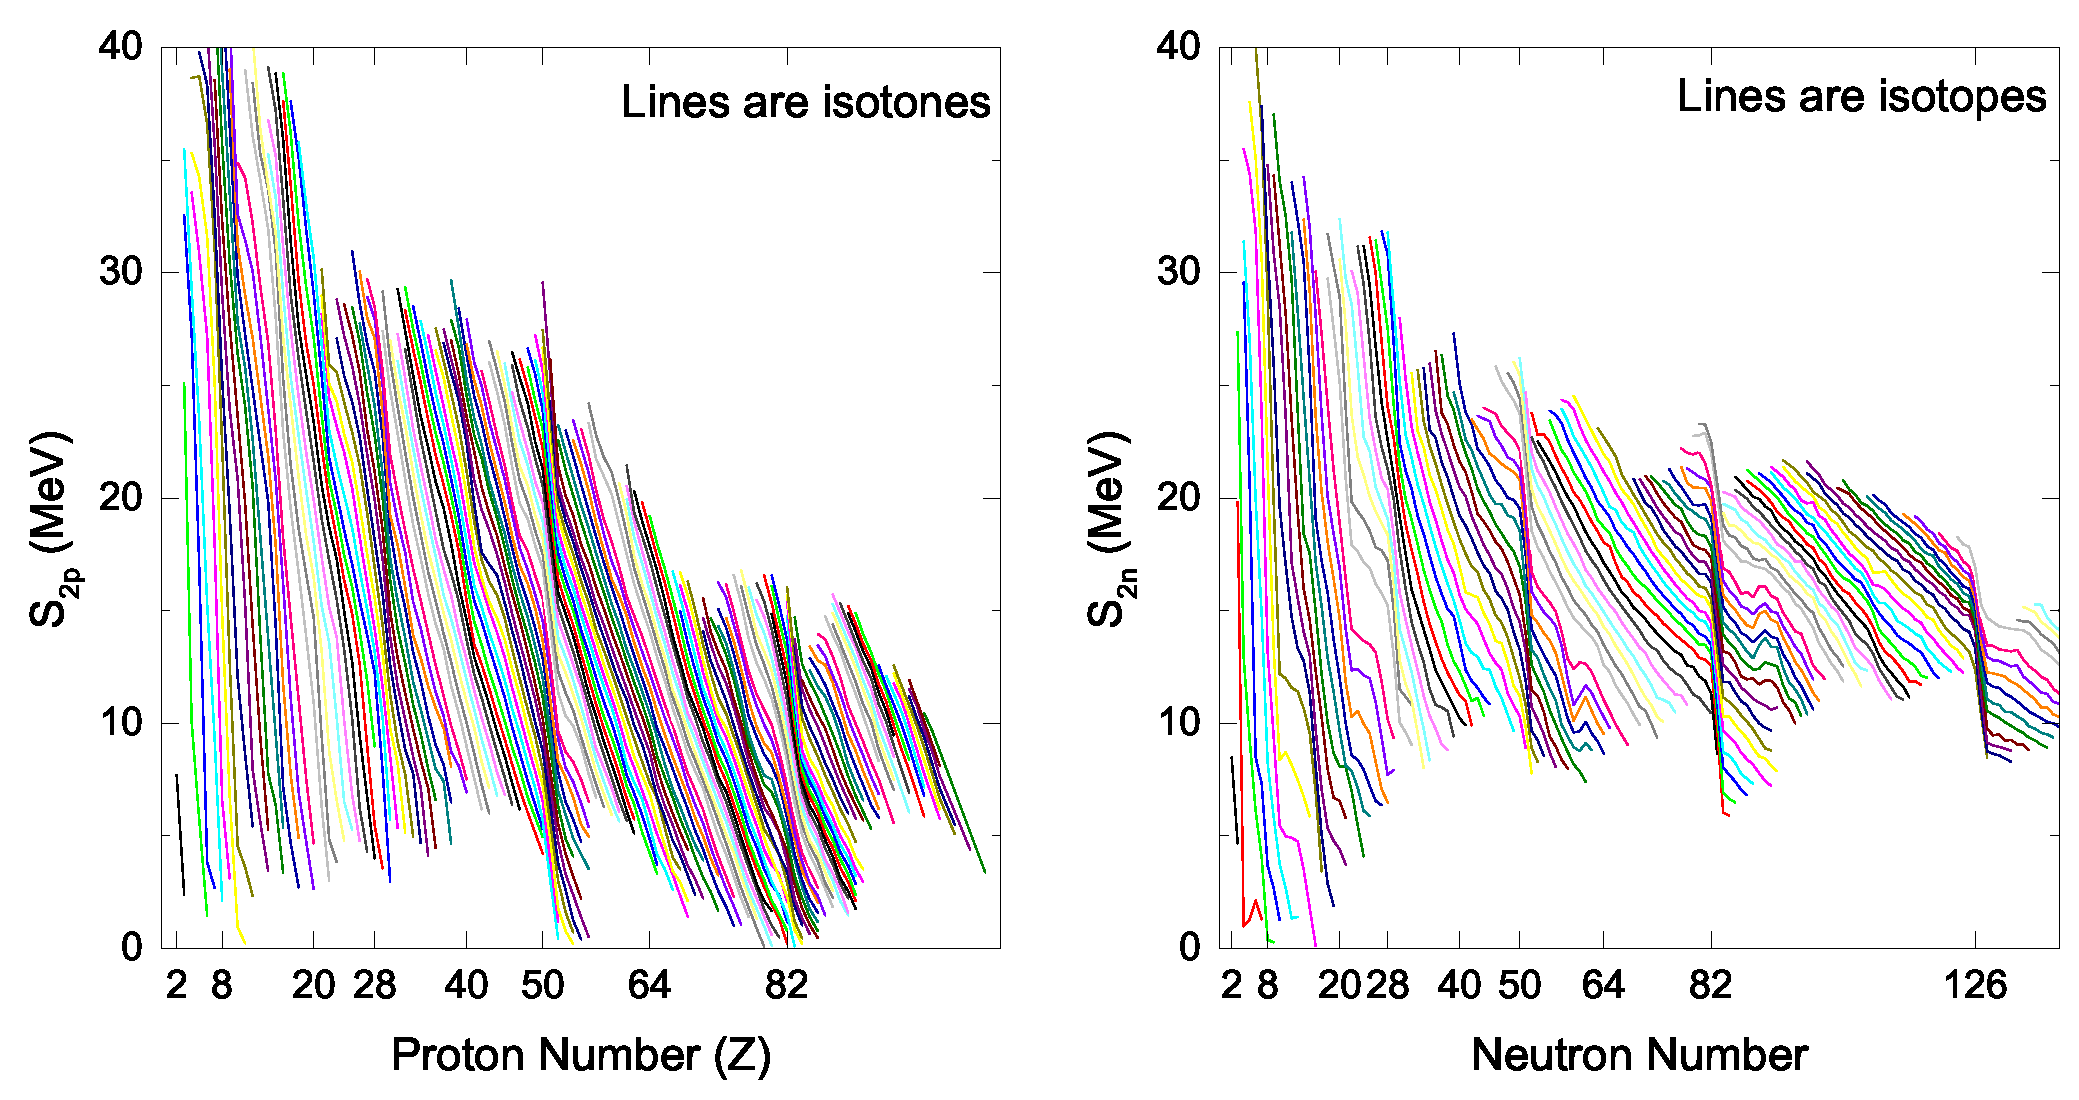
\includegraphics[width=\textwidth]{./img/c2/2nuc_sep_en.eps}}
	\caption{Left: Two proton separation energies plotted versus proton number. Each line is a set of isotones. Right: Two neutron separation energies plotted versus neutron number. Each line is a set of isotopes. Values calculated from: Ref.\cite{AME20031,AME20032}}
\end{figure}

\begin{figure}
\label{fig:chp2-two-plus-energies}
\centerline{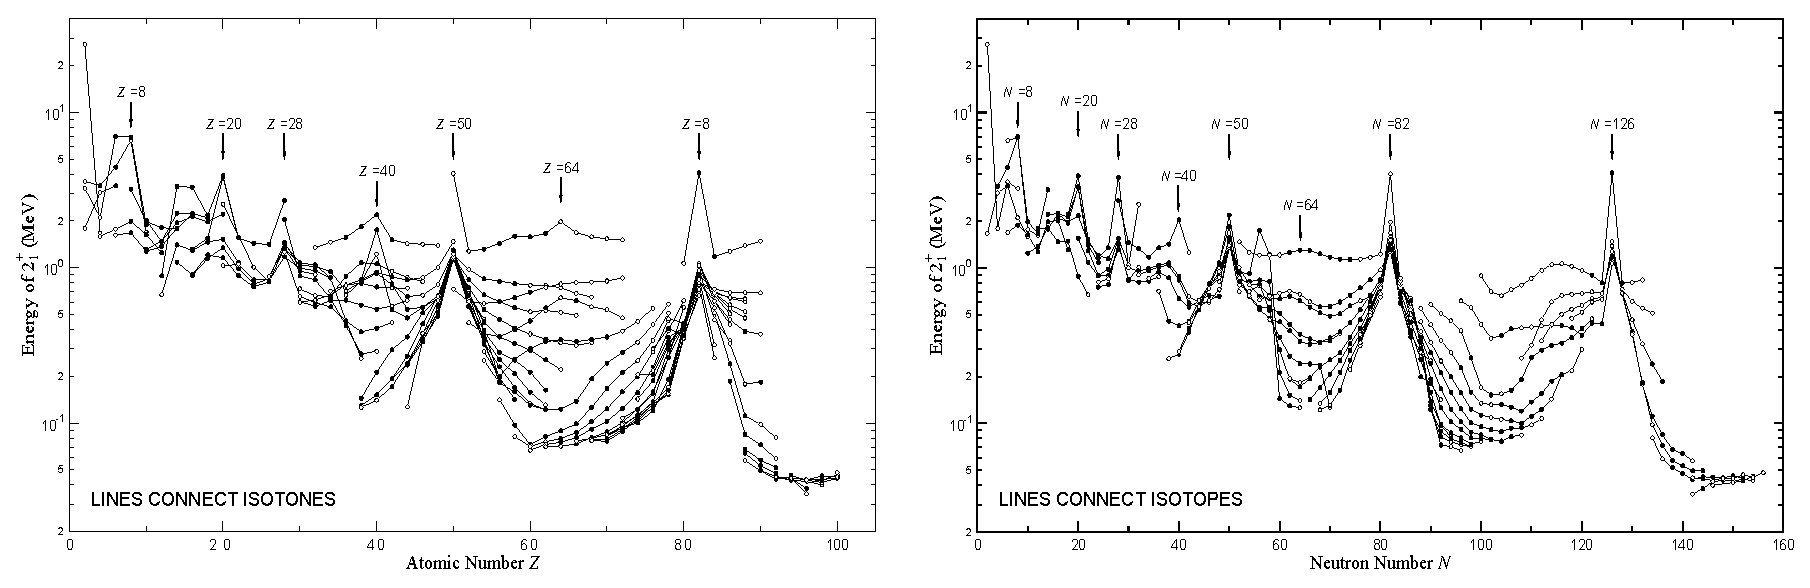
\includegraphics[width=\textwidth]{./img/c2/2_plus_en.eps}}
	\caption{Left: First excited $2^+$ energies of nuclei with even Z and N, plotted versus proton number. Each line is a set of isotones. Right: First excited $2^+$ energies of nuclei with even Z and N, plotted versus neutron number. Each line is a set of isotopes. Figures adapted from: Ref.\cite{RamanTwoPlus}}
\end{figure}

These magic numbers, occur at $2$, $8$, $20$, $28$, $50$, $82$, and $126$, though the proton shell closure corresponding to the neutron shell closure at $126$ is expected to be somewhat lower. The values $40$ and $60$ are also weakly magic over certain ranges of N and Z. These numbers can be derived from the calculation of a single particle in a mean field potential. While it is well known that the nuclear force is finite range with a shape similar to a Woods-Saxon potential, the Simple Harmonic Oscillator (SHO) potential is a reasonable first order approximation as seen in Figure \ref{fig:chp2-SHOPot}. Placing single particles in the SHO potential gives the first few magic numbers observed, however to reproduce the remaining magic numbers it is necessary to add a centrifugal $\vec{l}^2$ potential and a spin-orbit ($\vec{l}\cdot\vec{s}$ potential. This is shown in Figure \ref{fig:chp2-shell-model}.

\begin{figure}[h!]
\label{fig:chp2-SHOPot}
\centerline{\includegraphics[height=0.3\textheight]{./img/c2/sho_approx.png}}
	\caption{Schematic of a square well, SHO potential, and a realistic Woods-Saxon potential. Figure adapted from: Ref.\cite{casten}}
\end{figure}

\begin{figure}[h!]
\label{fig:chp2-shell-model}
\centerline{\includegraphics[height=0.8\textheight]{./img/c2/shell_model.png}}
	\caption{Spectrum of a single nucleon in an SHO potential, SHO + centrifugal potential, and, finally, SHO + centrifugal + spin-orbit. Figure adapted from: Ref.\cite{casten}}
\end{figure}

\subsection{The Deformed Shell Model}
\label{ssec:models-shell-model-def-sm}
\section{Rigid Rotor Model}
\label{sec:models-rigid-rotor}

\section{Tilted Axis Cranking}
\label{sec:models-tac}

\section{Wobbling Vibrations in Nuclei}
\label{sec:models-wobbling}
\subsection{Quasiparticle Triaxial Rotor (QTR)}
\label{sec:models-qtr}
\subsection{Signatures of Wobbling}
\label{sec:models-sig}
